\documentclass[12pt, orivec]{article}
\usepackage{amsmath}
\usepackage{amssymb}     % for \rightsquigarrow
\usepackage{wasysym}
\usepackage[breakable]{tcolorbox}
\usepackage{ulem}
\usepackage{tikz-cd}		% commutative diagrams
\usepackage{tikz}
\usepackage{amsthm}

\newtheorem{theorem}{Theorem}

\ifdefined\chinchin
\usepackage{xeCJK}
\setCJKmainfont[BoldFont=SimHei,ItalicFont=AR PL KaitiM GB]{SimSun}
\newcommand{\cc}[2]{#1}
\else
\newcommand{\cc}[2]{#2}
\fi

\newcommand{\code}   [1]{{\footnotesize{\ttfamily #1}}}
\newcommand{\tab}{\hspace*{2cm}}

\title{《计算范畴论》导读}
\author{甄景贤}

\begin{document}
\setlength{\parindent}{0pt}
\setlength{\parskip}{2.8ex plus0.8ex minus0.8ex}

\maketitle

恶补数学好几年之后,最近看懂了很多书。 《Computational category theory》 
是 Rydeheard \& Burstall 1988 年的书,但至今还没有类似的课本。  

我觉得这本书非常重要,因为它涉及到 \textbf{unification algorithm}。  现时人工智能中最关键的问题似乎是如何从 propositional logic(命题逻辑)过渡到 relational 或 first-order logic(一阶谓词逻辑),特别是如何找到高效率的学习算法。  关於 logic-based AI 的基础可以看看《AI --- a modern approach》 这本书。  

Unification algorithm(同一化算法)是 谓词逻辑 推导的核心算法。  将这个算法加进 命题逻辑 的推导算法(它叫消解法,resolution),就可以得到 谓词逻辑 的推导算法。  换句话说: unification + resolution = first-order deduction.

Unify 的意思是: 将两个 \textbf{逻辑项},透过 \textbf{variable substitution} 变成「一样」。  Variable substitution 是 谓词逻辑 的本质,\textbf{量词} $\forall$ 和 $\exists$ 就是作用在这些变量上。  所有初中生都懂得如何做「变量代入」,但它其实是一个很麻烦的动作,没有了它,谓词逻辑就变成命题逻辑。  虽然所有数学家都知道什么是 variable substitution,但它的精确描述,到了 1920-30 年代才开始出现。 例如 Sch\"{o}nfinkel 和 Curry 创造了 combinatory logic,Church 创造了 $\lambda$-calculus),他们的目的之一就是揭示「代入」的机制。 

Unification 的例子:
\begin{equation}
\mbox{loves}(X,Y) = \mbox{loves}(\mbox{john}, \mbox{mary}) \quad \mbox{ with } \{ X/\mbox{john}, Y/\mbox{mary} \}
\end{equation}
(如果逻辑里面有 function symbols 可以更复杂)

Unifcation 算法最初由 Jacques Herbrand (1930) 提出,后经 J A Robinson (1965) 发明 resolution 算法,再将它们结合,应用到自动推理。 
\begin{equation}
\vcenter{\hbox{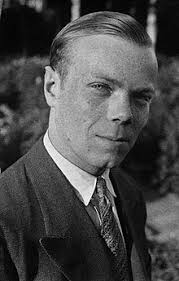
\includegraphics[scale=0.6]{Jacques-Herbrand.jpg}}} \quad
\vcenter{\hbox{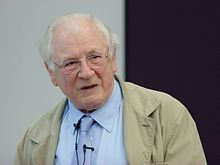
\includegraphics[scale=1.0]{John_Alan_Robinson.jpg}}} \nonumber
\end{equation}

在经典逻辑 AI 中,unification 是核心算法之一,但它的时间复习性并不是瓶颈。  笔者曾经研发过 higher-order unification,有开源代码在 GitHub.

以下是一个简单的 unification algorithm in Lisp,作者是 Peter Norvig: 
\begin{tcolorbox}[breakable]
\footnotesize
\ttfamily
\begin{verbatim}
;;; -*- Mode: Lisp; Syntax: Common-Lisp; -*-
;;; Code from Paradigms of Artificial Intelligence Programming
;;; Copyright (c) 1991 Peter Norvig

;;;; File unify.lisp: Unification functions

(requires "patmatch")

(defparameter *occurs-check* t "Should we do the occurs check?")

(defun unify (x y &optional (bindings no-bindings))
  "See if x and y match with given bindings."
  (cond ((eq bindings fail) fail)
        ((eql x y) bindings)
        ((variable-p x) (unify-variable x y bindings))
        ((variable-p y) (unify-variable y x bindings))
        ((and (consp x) (consp y))
         (unify (rest x) (rest y) 
                (unify (first x) (first y) bindings)))
        (t fail)))

(defun unify-variable (var x bindings)
  "Unify var with x, using (and maybe extending) bindings."
  (cond ((get-binding var bindings)
         (unify (lookup var bindings) x bindings))
        ((and (variable-p x) (get-binding x bindings))
         (unify var (lookup x bindings) bindings))
        ((and *occurs-check* (occurs-check var x bindings))
         fail)
        (t (extend-bindings var x bindings))))

(defun occurs-check (var x bindings)
  "Does var occur anywhere inside x?"
  (cond ((eq var x) t)
        ((and (variable-p x) (get-binding x bindings))
         (occurs-check var (lookup x bindings) bindings))
        ((consp x) (or (occurs-check var (first x) bindings)
                       (occurs-check var (rest x) bindings)))
        (t nil)))

(defun subst-bindings (bindings x)
  "Substitute the value of variables in bindings into x,
  taking recursively bound variables into account."
  (cond ((eq bindings fail) fail)
        ((eq bindings no-bindings) x)
        ((and (variable-p x) (get-binding x bindings))
         (subst-bindings bindings (lookup x bindings)))
        ((atom x) x)
        (t (reuse-cons (subst-bindings bindings (car x))
                       (subst-bindings bindings (cdr x))
                       x))))

(defun unifier (x y)
 "Return something that unifies with both x and y (or fail)."
 (subst-bindings (unify x y) x))
\end{verbatim}
\normalsize
\rmfamily
\end{tcolorbox}

从深度学习的角度考虑,问题是如何将 神经网络 算法 融合到 逻辑算法?  \uline{表面上看,这是两件截然不同的东西}。 笔者思考这个问题很多年,也提出过一些方案,但并不特别成功。 为了更明白 unification 的机制,我看了一些从范畴论角度处理 unification 的理论。

最早用范畴论角度研究 unification 的人是 Joseph Goguen (1941-2006),他发现了 unification 对应於范畴论中的 \textbf{co-equalizer} 概念:
\begin{equation}
\vcenter{\hbox{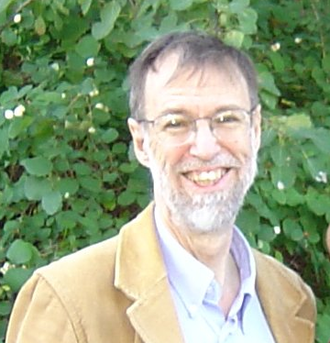
\includegraphics[scale=0.5]{Joseph-Goguen.png}}} \nonumber
\end{equation}
他写了一篇很详细的论文《What is unification? --- a categorical view of substitution, equation and solution》 (1989).

首先介绍一下什么是 \textbf{计算} 范畴论。  范畴论很抽象(它关注在集合之间的\textbf{映射},而不是集合里面的\textbf{元素}),但计算是具体的。  关键是: 用 \textbf{types} 代表 范畴论里的 objects,\textbf{functions} 代表范畴论里的 morphisms。  换句话说,用 \textbf{函数式编程} 模拟范畴论。

\begin{tcolorbox}
众所周知,Haskell 的前身是 ML,ML = Lisp + type system.  ML 也衍生了 OCaml = Objective Caml,而 Caml 的 CAM = categorical abstract machine.  CAM 是 Cartesian-closed category 和 combinatory logic 的结合。 (我暂时还不大清楚 CAM 的理论)
\end{tcolorbox}

在 Rydeheard \& Burstall 这本书里,用的语言是 ML。 例如: \\
\tab 用 type \code{`o} 表示 objects,\\
\tab 用 type \code{`a} 表示 arrows,\\
那么 source 和 target 函数的类型就是 \\
\tab \code{`a -> `o}.

范畴论中,\textbf{co-equalizer} 的定义是:
\begin{equation}
\begin{tikzcd}
X \ar[r,shift left=.75ex,"f"]
  \ar[r,shift right=.75ex,swap,"g"]
&
Y \ar[r,"q"] \ar[dr,swap,"q'"]
&
Q \ar[d,densely dashed, "!"]
\\
& & Q'
\end{tikzcd}
\end{equation}
换句话说,$q$ 是唯一的箭咀,令 $qf = qg$.

它的\textbf{对偶},\textbf{equalizer} 的定义,三角形在左边:
\begin{equation}
\begin{tikzcd}
Q \ar[r,"q"]
&
X \ar[r,shift left=.75ex,"f"]
  \ar[r,shift right=.75ex,swap,"g"]
&
Y
\\
Q' \ar[ur,"q'"]
   \ar[u,densely dashed, "!"]
 & &
\end{tikzcd}
\end{equation}
其中 $fq = gq$.

它们的意义不相同:

\uline{An \textbf{equalizer} is a generalization of the idea of the \textbf{kernel} of a homomorphism, or an equationally defined ``variety'', like the zero-set of a real-valued function}.

\uline{A \textbf{co-equalizer} is a generalization of a \textbf{quotient} by an equivalence relation}.

在此只解释 co-equalizer:  Define a relation on $Y$ by $y_1 \rightsquigarrow y_2$ iff $\exists x \in X$ such that $f(x) = y_1$ and $g(x) = y_2$.  Let $\simeq$ be the equivalence closure of $\rightsquigarrow$, and $Q$ be the set of $\simeq$-equivalence classes.  The quotient function $q: Y \rightarrow Q$ maps an element $y$ to its equivalence class $[y]$ so that $qf = qg$.

在 R \& B 书中 \S 3.4.2 讲述了 逻辑 \textbf{terms} 的范畴 $\mathcal{T}_{\Omega}(X)$,其中 $X$ 是 the set of variables。  A \textbf{term substitution} $f: X \rightarrow Y$ 是作用到这个范畴内的函数:
\begin{equation}
f: X \rightarrow \mathcal{T}_{\Omega}(Y)
\end{equation}

Unification 作用在一些形如 $s = t$ 的 \textbf{equations} 上。

假设有一组 equations 用 index set $I$ 指标: $\{ s_i = t_i : i \in I \}$.  这组等式可以这样表示:
\begin{equation}
\begin{tikzcd}
I \ar[r,shift left=.75ex,"f"]
  \ar[r,shift right=.75ex,swap,"g"]
& X
\end{tikzcd}
\end{equation}
where $f(i) = s_i, g(i) = t_i$.  换句话说 $f$ 和 $g$ 分别指向 \uline{等式的左右两端}。

基於范畴论的算法的特点是: \uline{将函数 recursively \textbf{分拆} 成更细小的函数来计算}。 

\begin{theorem}
If $q: X \rightarrow Q$ is the co-equalizer of the parallel pair:
\begin{equation}
\begin{tikzcd}
I \ar[r,shift left=.75ex,"f"]
  \ar[r,shift right=.75ex,swap,"g"]
& X \ar[r, "q"] & Q
\end{tikzcd}
\end{equation}
and $r: Q \rightarrow R$ is the co-equalizer:
\begin{equation}
\begin{tikzcd}
& X \ar[dr, "q"] & \\
I' \ar[ur, "f'"]
   \ar[dr, "g'"]
& & Q \ar[r, "r"] & R\\
& X \ar[ur,"q"] &
\end{tikzcd}
\end{equation}
then $rq:  X \rightarrow R$ is the co-equalizer:
\begin{equation}
\begin{tikzcd}
I + I' \arrow[shift left=.75ex]{r}{[f, f']}
       \arrow[shift right=.75ex,swap]{r}{[g, g']}
& X \ar[r, "rq"] & R
\end{tikzcd}
\end{equation}
\end{theorem}

这分拆的意思是,例如: 
\begin{equation}
\mbox{loves}(X, Y) = \mbox{loves}(\mbox{john}, \mbox{mary})
\end{equation}
则分拆成两条 equations:
\begin{eqnarray}
X &=& \mbox{john} \\
Y &=& \mbox{mary}
\end{eqnarray}

另外还有一个 theorem 将 term 分拆出 \textbf{sub-term},在书里有解释,从略。 



\end{document}